% !TEX TS-program = pdflatex
% !TEX encoding = UTF-8 Unicode

% This is a simple template for a LaTeX document using the "article" class.
% See "book", "report", "letter" for other types of document.

\documentclass[11pt]{article} % use larger type; default would be 10pt


%%% PAGE DIMENSIONS
%\usepackage{geometry} % to change the page dimensions
%\geometry{a4paper} % or letterpaper (US) or a5paper or....
% \geometry{margin=2in} % for example, change the margins to 2 inches all round
% \geometry{landscape} % set up the page for landscape
%   read geometry.pdf for detailed page layout information
%\usepackage[textwidth=14cm,textheight=20cm]{geometry}
\usepackage[a4paper,%
            left=2.5cm,right=2.5cm,top=2.5cm,bottom=2.5cm,%
            footskip=.6cm]{geometry}

\def\changemargin#1#2{\list{}{\rightmargin#2\leftmargin#1}\item[]}
\let\endchangemargin=\endlist


\usepackage{graphicx} % support the \includegraphics command and options
\usepackage[parfill]{parskip} % Activate to begin paragraphs with an empty line rather than an indent


%%% PACKAGES
\usepackage{booktabs} % for much better looking tables
\usepackage{array} % for better arrays (eg matrices) in maths
\usepackage{paralist} % very flexible & customisable lists (eg. enumerate/itemize, etc.)
\usepackage{verbatim} % adds environment for commenting out blocks of text & for better verbatim
\usepackage{subfig} % make it possible to include more than one captioned figure/table in a single float
% These packages are all incorporated in the memoir class to one degree or another...


\usepackage{float}
\usepackage[all]{xy}
\usepackage{booktabs}
\usepackage{makecell}
\usepackage{enumerate}
\usepackage{scrextend}
\usepackage{mathtools}
\usepackage{yfonts}
\usepackage{setspace} 

\title{\LARGE Seminar zum Thema Numerische multilineare Algebra:\\
\LARGE Tensor Spaces and Numerical Tensor Calculus\\
\vspace{5mm} %5mm vertical space
\large Vortrag: Numerische Verfahren zur Bestimmung des Rangs eines Tensors}

\date{Vortrag vom 13.01.2020}

\author{Tibor Gr{\"u}n}


\makeatletter
% we use \prefix@<level> only if it is defined
\renewcommand{\@seccntformat}[1]{%
  \ifcsname prefix@#1\endcsname
    \csname prefix@#1\endcsname
  \else
    \csname the#1\endcsname\quad
  \fi}
% define \prefix@section
\newcommand\prefix@section{Kapitel \thesection: }
\makeatother


%%% For Math
\usepackage{amsmath}
\usepackage{amsfonts}
\usepackage{amsbsy}
\usepackage{amsthm}
\usepackage{amssymb}

\makeatletter
\renewcommand*\env@matrix[1][*\c@MaxMatrixCols c]{%
  \hskip -\arraycolsep
  \let\@ifnextchar\new@ifnextchar
  \array{#1}}
\makeatother

%%% Math theorem styles

\newtheorem{thm}{Satz}[section]
\newtheorem{lemma}[thm]{Lemma}
\theoremstyle{definition}
\newtheorem{definition}[thm]{Definition}
\newtheorem{rmk}[thm]{Bemerkung}
\newtheorem{alg}[thm]{Algorithmus}


%%% For graphics
\usepackage{tikz}
\usepackage{pgfbaselayers}

\pgfdeclarelayer{background}
\pgfdeclarelayer{foreground}
\pgfsetlayers{background,main,foreground}



%\DeclareMathOperator{\Hom}{Hom}
%\DeclareMathOperator{\dom}{dom}
%\DeclareMathOperator{\codom}{codom}

\begin{document}
\maketitle

\section{Tensoren}

\subsection{Was ist ein Tensor?}

\subsubsection{Vektoren, Matrizen, Tensoren: Grafische Darstellung}

[Abbildungen]

\subsubsection{Multi-Index, \textit{d}-stufiger Tensorraum}

\begin{definition} (Multi-Index)
\end{definition}

\begin{rmk} (Ordnung auf $\mathbb{N}_{0}^{d}$)
\end{rmk}

\begin{definition} ($\mathbb{R}^{\mathbf{I}}$)
\end{definition}

\begin{rmk} ($n^{d}$ ist viel)
\end{rmk}

\subsubsection{Das Tensorprodukt $\otimes$ als Beziehung zwischen $\mathbb{R}^{\mathbf{I}}$ und den $\mathbb{R}^{I_{j}}$}

\begin{definition} ($\otimes$ für Vektoren)
\end{definition}

\begin{definition} ($\otimes$ für Vektorräume)
\end{definition}

\begin{lemma} (Gleichheit der Tensorräume)
\end{lemma}
\begin{proof}[\underline{Beweis:}\nopunct]

\end{proof}

\subsubsection{Tensoren als Multilineare Abbildungen: Universalität des Tensorprodukts}

\subsubsection{Beispiel $d=2$ : Matrizen als Tensoren}

\subsubsection{Beispiel $d=3$ : Graustufen-Film: Höhe $\times$ Breite $\times$ Zeit }

\section{Tensordarstellung und Tensorzerlegung}

\subsection{Tensorrang und die Menge $\mathcal{R}_{r}$}

\begin{rmk} (nicht abgeschlossen für d $\geq 3$ und $r \geq 2$)
\end{rmk}

\begin{thm} (De Silva/Lim 2008)
\end{thm}
\begin{proof}[\underline{Beweis:}\nopunct]
\end{proof}


\subsection{Tucker-Rang und Tucker-Zerlegung: Die Menge $\mathcal{T}_{\mathbf{r}}$}

\subsubsection{Unterräume $U_{j}$ und minimale Unterräume $U_{j}^{\min}$}

\begin{rmk} (\textbf{Tucker-Rang})
\end{rmk}

\subsection{Approximierung}

\begin{rmk} (weakly closed)
\end{rmk}

\begin{alg} (ALS)
\end{alg}

\subsubsection{Beispiel: Tucker-Zerlegung eines 5-stufigen Tensors}


%
% tensor T
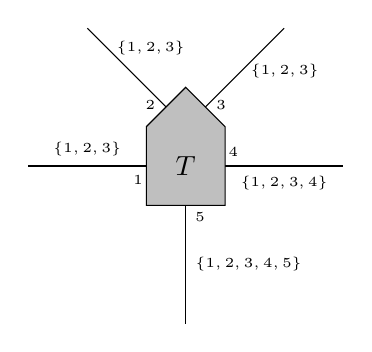
\begin{tikzpicture}
\begin{pgfonlayer}{foreground}
\draw[fill=lightgray] (0-0.5cm,0-0.5cm) -- (0+0.5cm,0-0.5cm) -- (0+0.5cm,0+0.5cm) -- (0,0+1cm) -- (0-0.5cm,0+0.5cm) -- cycle;
\node at (0,0) {$T$};
\end{pgfonlayer}
\begin{pgfonlayer}{background}
\draw[-] (0-0.5cm,0) -- node [below,pos=0.07] {\tiny1} node [above,midway] {\tiny$\{1,2,3\}$} (0-2cm,0); %j=1
\draw[-] (0-0.25cm,0+0.75cm) -- node [below,pos=0.2] {\tiny2} node [right,near end] {\tiny$\{1,2,3\}$} (0-1.25cm,0.5cm+1.25cm); %j=2
\draw[-] (0+0.25cm,0+0.75cm) -- node [below,pos=0.2] {\tiny3} node [right,pos=0.45] {\tiny$\{1,2,3\}$} (0+1.25cm,0.5cm+1.25cm); %j=3
\draw[-] (0+0.5cm,0) -- node [above,pos=0.07] {\tiny4} node [below,midway] {\tiny$\{1,2,3,4\}$} (0+2cm,0); %j=4
\draw[-] (0,0-0.5cm) -- node [right,pos=0.1] {\tiny5} node [right,midway] {\tiny$\{1,2,3,4,5\}$} (0,-0.5cm-1.5cm); %j=5
\end{pgfonlayer}
\end{tikzpicture}

%
% core tensor X
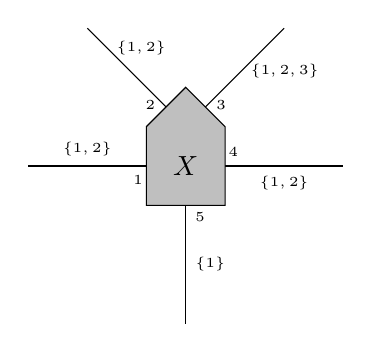
\begin{tikzpicture}
\begin{pgfonlayer}{foreground}
\draw[fill=lightgray] (0-0.5cm,0-0.5cm) -- (0+0.5cm,0-0.5cm) -- (0+0.5cm,0+0.5cm) -- (0,0+1cm) -- (0-0.5cm,0+0.5cm) -- cycle;
\node at (0,0) {$X$};
\end{pgfonlayer}
\begin{pgfonlayer}{background}
\draw[-] (0-0.5cm,0) -- node [below,pos=0.07] {\tiny1} node [above,midway] {\tiny$\{1,2\}$} (0-2cm,0); %j=1
\draw[-] (0-0.25cm,0+0.75cm) -- node [below,pos=0.2] {\tiny2} node [right,near end] {\tiny$\{1,2\}$} (0-1.25cm,0.5cm+1.25cm); %j=2
\draw[-] (0+0.25cm,0+0.75cm) -- node [below,pos=0.2] {\tiny3} node [right,pos=0.45] {\tiny$\{1,2,3\}$} (0+1.25cm,0.5cm+1.25cm); %j=3
\draw[-] (0+0.5cm,0) -- node [above,pos=0.07] {\tiny4} node [below,midway] {\tiny$\{1,2\}$} (0+2cm,0); %j=4
\draw[-] (0,0-0.5cm) -- node [right,pos=0.1] {\tiny5} node [right,midway] {\tiny$\{1\}$} (0,-0.5cm-1.5cm); %j=5
\end{pgfonlayer}
\end{tikzpicture}

% 
% core tensor X with matrices U1,...,U5
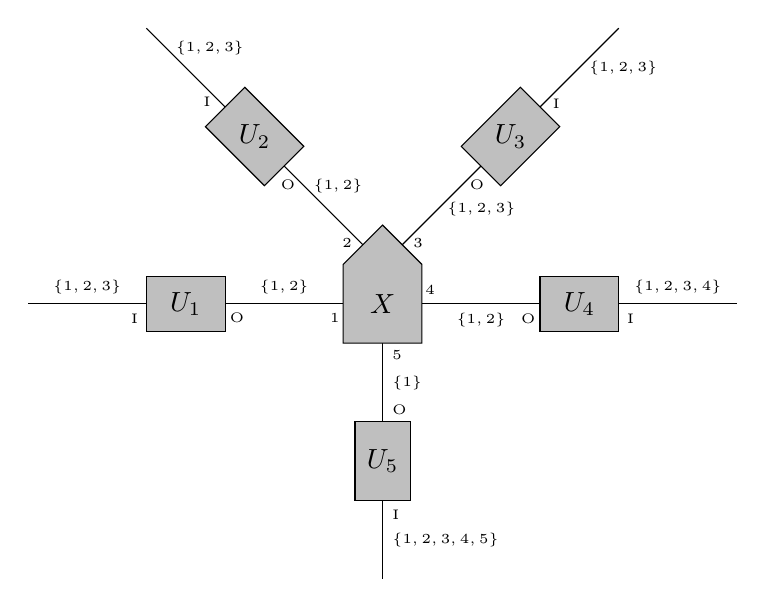
\begin{tikzpicture}
\begin{pgfonlayer}{foreground}
\draw[fill=lightgray] (0-0.5cm,0-0.5cm) -- (0+0.5cm,0-0.5cm) -- (0+0.5cm,0+0.5cm) -- (0,0+1cm) -- (0-0.5cm,0+0.5cm) -- cycle;
\node at (0,0) {$X$};
\end{pgfonlayer}
\begin{pgfonlayer}{background}
\draw[-] (0-0.5cm,0) -- node [below,pos=0.9] {\tiny O} node [below,pos=0.07] {\tiny1} node [above,midway] {\tiny$\{1,2\}$} (0-2cm,0); %j=1
\draw[-] (0-0.25cm,0+0.75cm) -- node [below,pos=0.95] {\tiny O} node [below,pos=0.2] {\tiny2} node [right,near end] {\tiny$\{1,2\}$}
 (0-1.25cm,0.5cm+1.25cm); %j=2
\draw[-] (0+0.25cm,0+0.75cm) -- node [below,pos=0.95] {\tiny O} node [below,pos=0.2] {\tiny3} node [right,pos=0.45] {\tiny$\{1,2,3\}$} 
(0+1.25cm,0.5cm+1.25cm); %j=3
\draw[-] (0+0.5cm,0) -- node [below,pos=0.9] {\tiny O} node [above,pos=0.07] {\tiny4} node [below,midway] {\tiny$\{1,2\}$} 
(0+2cm,0); %j=4
\draw[-] (0,0-0.5cm) -- node [right,pos=0.85] {\tiny O} node [right,pos=0.15] {\tiny5} node [right,midway] {\tiny$\{1\}$} 
(0,-0.5cm-1cm); %j=5
\end{pgfonlayer}
%U1 p=(-2.5cm,0)
\draw[fill=lightgray] (-2.5cm-0.5cm,0-0.35cm) -- (-2.5cm+0.5cm,0-0.35cm) -- (-2.5cm+0.5cm,0+0.35cm) -- (-2.5cm-0.5cm,0+0.35cm) -- cycle;
\node at (-2.5cm,0) {$U_{1}$};
\draw[-] (-2.5cm-0.5cm,0) -- node [below,pos=0.1] {\tiny I} node [above,midway] {\tiny$\{1,2,3\}$} (-2.5cm-2cm,0);
%U2 p=(-1.5cm,2cm)
\draw[fill=lightgray] (-1.5cm,2cm-0.5cm) -- (-1.5cm-0.75cm,2cm-0.5cm+0.75cm) -- (-1.5cm-0.25cm,2cm+0.75cm) -- (-1.5cm+0.5cm,2cm) -- cycle;
\node at (-1.5cm-0.125cm,2cm+0.125cm) {$U_{2}$};
\draw[-] (-2cm,2.5cm) -- node [left,pos=0.06] {\tiny I} node [right,near end] {\tiny$\{1,2,3\}$} (-3cm,3.5cm);
%U3 p=(1.5cm,2cm)
\draw[fill=lightgray] (1.5cm-0.5cm,2cm) -- (1.5cm+0.25cm,2cm+0.75cm) -- (1.5cm+0.75cm,2cm+0.25cm) -- (1.5cm,2cm-0.5cm) -- cycle;
\node at (1.5cm+0.125cm,2cm+0.125cm) {$U_{3}$};
\draw[-] (1.5cm+0.5cm,2cm+0.5cm) -- node [right,pos=0.04] {\tiny I} node [right,midway] {\tiny$\{1,2,3\}$} (3cm,3.5cm);
%U4 p=(2.5cm,0)
\draw[fill=lightgray] (2.5cm-0.5cm,0-0.35cm) -- (2.5cm+0.5cm,0-0.35cm) -- (2.5cm+0.5cm,0+0.35cm) -- (2.5cm-0.5cm,0+0.35cm) -- cycle;
\node at (2.5cm,0) {$U_{4}$};
\draw[-] (2.5cm+0.5cm,0) -- node [below,pos=0.1] {\tiny I} node [above,pos=0.5] {\tiny$\{1,2,3,4\}$} (2.5cm+2cm,0);
%U5 p=(0,-2cm)
\draw[fill=lightgray] (0-0.35cm,-2cm+0.5cm) -- (0-0.35cm,-2cm-0.5cm) -- (0+0.35cm,-2cm-0.5cm) -- (0+0.35cm,-2cm+0.5cm) -- cycle;
\node at (0,-2cm) {$U_{5}$};
\draw[-] (0,-2.5cm) -- node [right,pos=0.18] {\tiny I}  node [right,midway] {\tiny$\{1,2,3,4,5\}$} (0,-3.5cm);
\end{tikzpicture}


\section{Octave-Demonstration von tucker\_als}

\end{document}
